\documentclass{beamer}
\usepackage[utf8]{inputenc}
\usepackage{graphicx}

\newtheorem{definicion}{Definición}
\newtheorem{ejemplo}{Ejemplo}

%%%%%%%%%%%%%%%%%%%%%%%%%%%%%%%%%%%%%%%%%%%%%%%%%%%%%%%%%%%%%%%%%%%%%%%%%%%%%%%
\title[Presentación con Beamer]{Series de potencias de Taylor }
\author[SCR]{Sergio Álvarez Fernández\\Cirilo Fleitas Rufino\\Rayco Hernández Delgado}
\date[16-05-2014]{16 de mayo de 2014}
%%%%%%%%%%%%%%%%%%%%%%%%%%%%%%%%%%%%%%%%%%%%%%%%%%%%%%%%%%%%%%%%%%%%%%%%%%%%%%%

%\usetheme{Madrid}
\usetheme{Antibes}
%\usetheme{tree}
%\usetheme{classic}

%%%%%%%%%%%%%%%%%%%%%%%%%%%%%%%%%%%%%%%%%%%%%%%%%%%%%%%%%%%%%%%%%%%%%%%%%%%%%%%
\begin{document}


  
%++++++++++++++++++++++++++++++++++++++++++++++++++++++++++++++++++++++++++++++
\begin{frame}

  %\includegraphics[width=0.15\textwidth]{img/ullesc}
  %\hspace*{7.0cm}
  %\includegraphics[width=0.16\textwidth]{img/fmatesc}
  \titlepage

  \begin{small}
    \begin{center}
     Facultad de Matemáticas \\
     Universidad de La Laguna
    \end{center}
  \end{small}

\end{frame}
%++++++++++++++++++++++++++++++++++++++++++++++++++++++++++++++++++++++++++++++

%++++++++++++++++++++++++++++++++++++++++++++++++++++++++++++++++++++++++++++++
\begin{frame}
  \frametitle{Índice}
  \tableofcontents[pausesections]
\end{frame}
%++++++++++++++++++++++++++++++++++++++++++++++++++++++++++++++++++++++++++++++


\section{Introducción a Taylor}
\begin{frame}

 \[f(x) = f(a)
  + \frac{f'(a)}{1!}(x - a)
  + \frac{f^{(2)}(a)}{2!}(x - a)^2
  + \cdots
  + \frac{f^{(n)}(a)}{n!}(x - a)^n
  + R_n(f)\]
  
\[f(x) = \sum_{k=0}^n \frac{f^{(k)}(a)}{k!}(x - a)^k + R_n(f)\]

\[R_n(f) = \frac{f^{(n+1)}(\xi)}{(n+1)!} (x-a)^{n+1}\]

\[R_n(f) = \int_a^x \frac{f^{(n+1)} (t)}{n!} (x - t)^n \, dt\]

\end{frame}


\section{Código python}

%++++++++++++++++++++++++++++++++++++++++++++++++++++++++++++++++++++++++++++++
\subsection{Cálculo polinomio de Taylor}
\label{}
\begin{frame}[fragile]
\begin{center}
\begin{tiny}
\begin{verbatim}

Errores=[0.4789, 0.0456, 0.00005, 0.000000005, 0.000000000007]
x=2.0
c=0.0
f=(x+c)/2

valor_c = Symbol('c')
valor_a = Symbol('f')
funcion = cos(valor_c)
funcion_ = cos (valor_a)

def fac(n):
  if n == 0:
    return 1
  else:
    return n * fac(n-1)

def MostrarTaylor(c,n):
  for i in range(n + 1):
    derivada = eval(str(diff(funcion,valor_c,i)))
    if (i<1):
     sys.stdout.write((str(derivada)))
    if(i>=1):
     x=Symbol('x')
     a=(derivada*((x-c)**i))
     if (derivada != 0):
       if (derivada<0):	 
        a=-a
        sys.stdout.write((' - '+str(a) +' / '+str (i)+'!'))
       else: 
        sys.stdout.write((' + '+str(a) +' / '+str (i)+'!'))
  print '\n' 
  return 
\end{verbatim}
\end{tiny}
\end{center}
\end{frame}
\begin{frame}[fragile]
\begin{center}
\begin{tiny}
\begin{verbatim}
def graficaTaylor(c,n):
 v=0
  for i in range(n + 1):
    derivada = eval(str(diff(funcion,valor_c,i)))
    if (i<1):
     v=v+derivada
    if(i>=1):
     x=np.arange(-10,10,0.001)
     a=(derivada*((x-c)**i))
     if (derivada != 0):
       v=v+derivada*((x-c)**i)/fac(i) 
  return v

def ErrorTaylor(x,c,error):
  i=0
  derivada = eval(str(diff(funcion_,valor_a,i)))
  polinomio = ((derivada/(fac(i)))*((x - c)**i))
  while (abs(polinomio)>=error):
    i+=1
    derivada = eval(str(diff(funcion_,valor_a,i)))
    polinomio = ((derivada/(fac(i)))*((x - c)**i))
  return i

if __name__=='__main__':
  for error in Errores:
    n=ErrorTaylor(x,c,error)
    print ('\n %3i iteraciones para dar un error <= %.15f') %(n,error)
    MostrarTaylor(c,n-1)
    
    
\end{verbatim}
\end{tiny}
\end{center}
\end{frame}

\subsection{Representación de gráficas}
\begin{frame}[fragile]
\begin{center}
\begin{tiny}
\begin{verbatim}
n=3
tiempo=[]
xtiempo=[]

graf1= plt.subplot(211)
print"Cargado el   0 por ciento de las Graficas"
i=0
for error in calculotaylor.Errores:
    start=time.time()
    i+=1
    n=calculotaylor.ErrorTaylor(calculotaylor.x,calculotaylor.c,error)
    x1=np.arange(-10,10,0.001)
    y=calculotaylor.graficaTaylor(calculotaylor.c,n)
    plt.plot(x1,y, label= 'n = %d' %(n-1))
    print"Cargado %3d por ciento de las Graficas" %(100*i/(len(calculotaylor.Errores))) # Calcula el % de los datos introducidos en el Grafica, así hace la espera mas amena.
    finish=time.time()-start
    tiempo=tiempo+[finish]
plt.plot(x1,np.cos(x1), label = 'cos(x)')    
plt.title('Series de Potencias de Taylor de grado n')
plt.legend(loc = 3) 
plt.ylim(-1.5,1.5)
for i in range (1,len(tiempo)+1):
  xtiempo=xtiempo+[i]
graf2=plt.subplot(212)
plt.title('Tiempo que tarda en calcular el Polinomio de Taylor')
plt.plot(xtiempo,tiempo, 'bo')
plt.xticks(xtiempo, size = 'small', color = 'b')
plt.yticks(tiempo, size = 'small', color = 'b')
plt.xlabel("Numero del error")
plt.ylabel("Tiempo")
plt.xlim(0,(len(tiempo)+1))
plt.savefig("Graficas.eps", dpi=100)
plt.show()
\end{verbatim}
\end{tiny}
\end{center}
\end{frame}


\section{Gráficas}
\begin{frame}
\frametitle{Cálculo de gráficas}
Errores utilizados e1 = 0.4789; e2 = 0.0456; e3 = 0.00005; e4 = 0.000000005; e5 = 0.000000000007
\begin{figure}[!th]
\begin{center}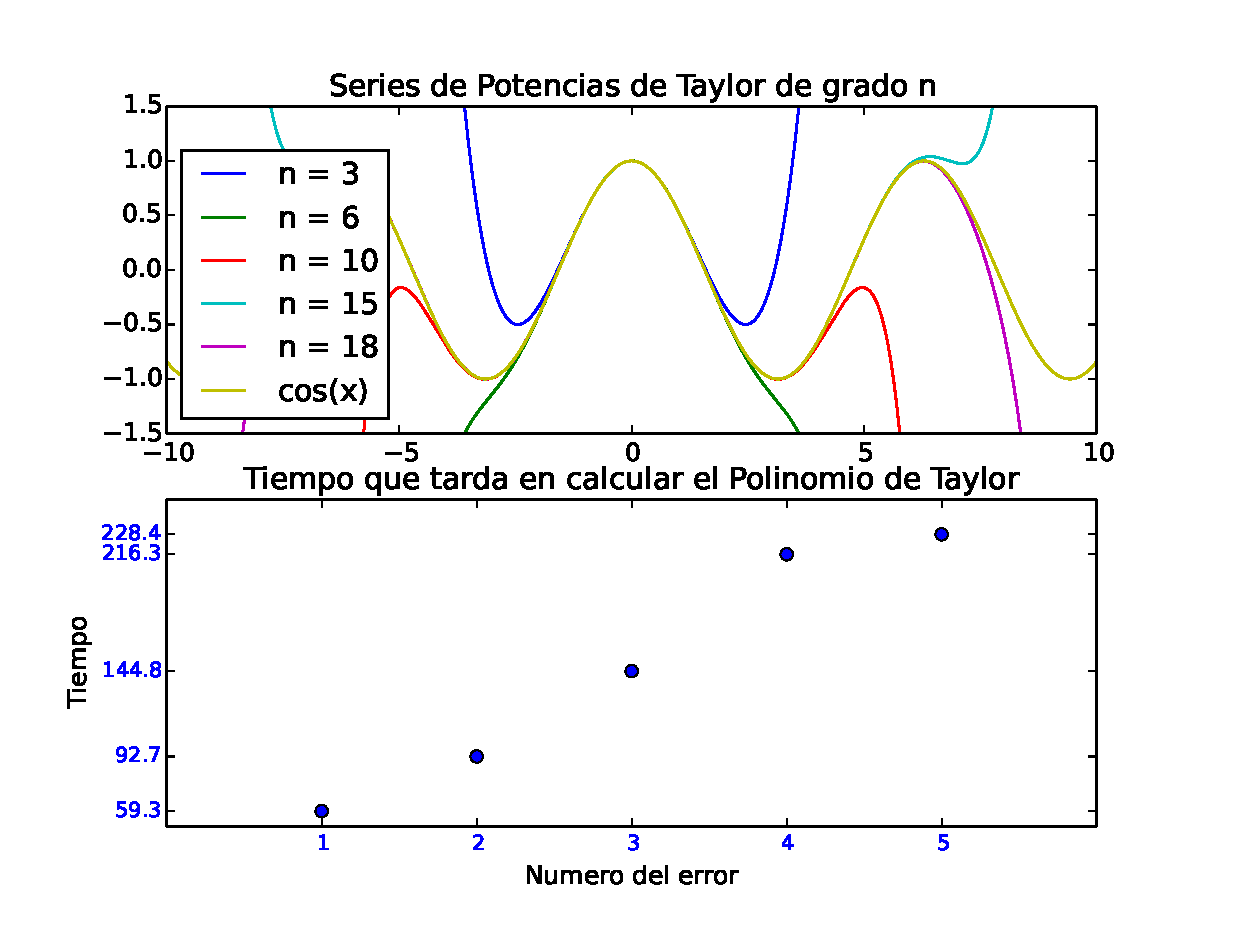
\includegraphics[height=5cm, width=6cm]{images/Graficas.eps}
\caption{centro = 0; x = 2}
\label{cos}
\end{center}
\end{figure} 

\end{frame}  

\begin{frame}
Errores utilizados e1 = 0.4789; e2 = 0.0456; e3 = 0.00005; e4 = 0.000000005; e5 = 0.000000000007
\begin{figure}[!th]
\begin{center}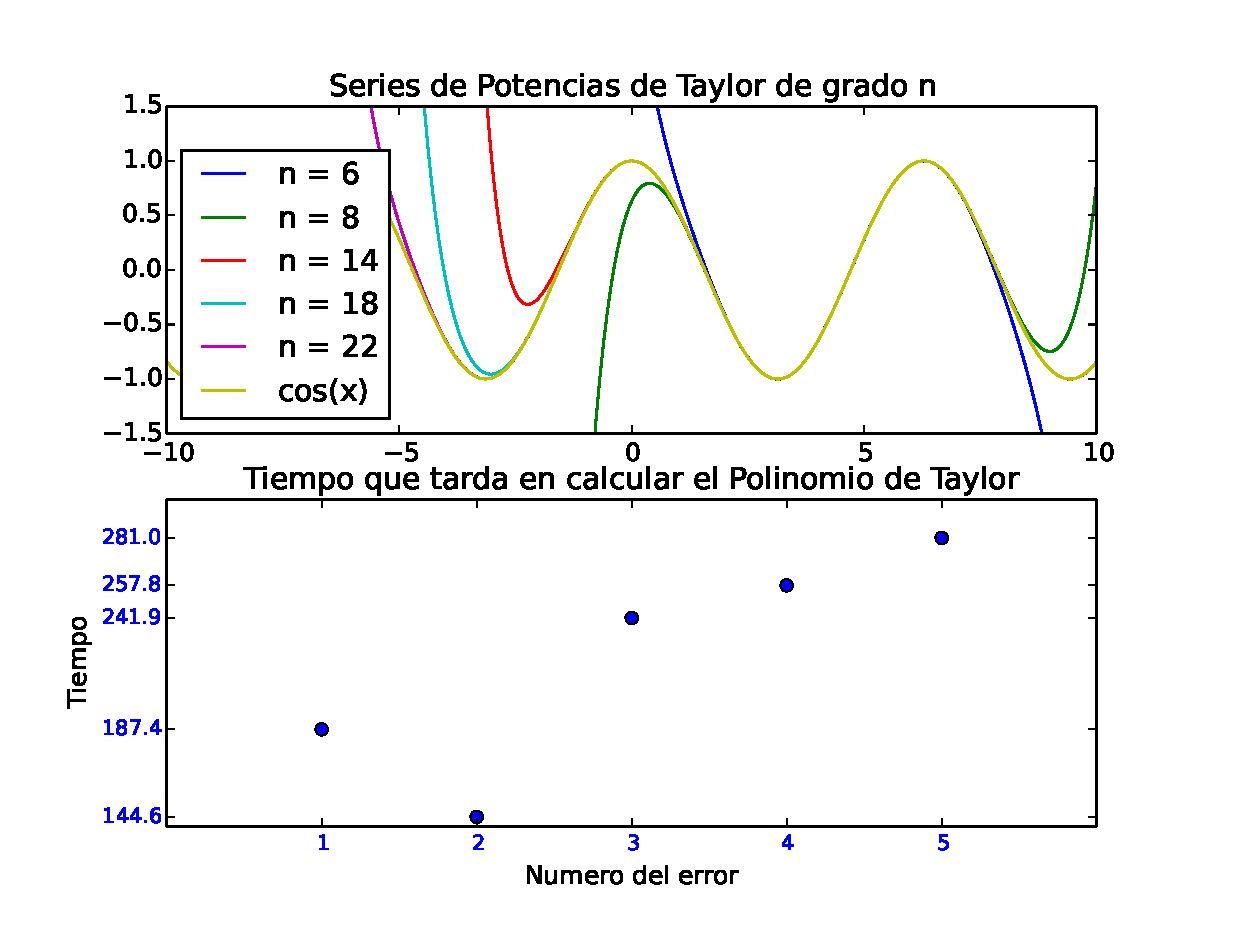
\includegraphics[height=5cm, width=6cm]{images/Graficascentro5.eps}
\caption{centro = 5; x = 2}
\label{cos}
\end{center}
\end{figure}

\end{frame}  

\begin{frame}
Errores utilizados e1 = 0.4789; e2 = 0.0456; e3 = 0.00005; e4 = 0.000000005; e5 = 0.000000000007
\begin{figure}[!th]
\begin{center}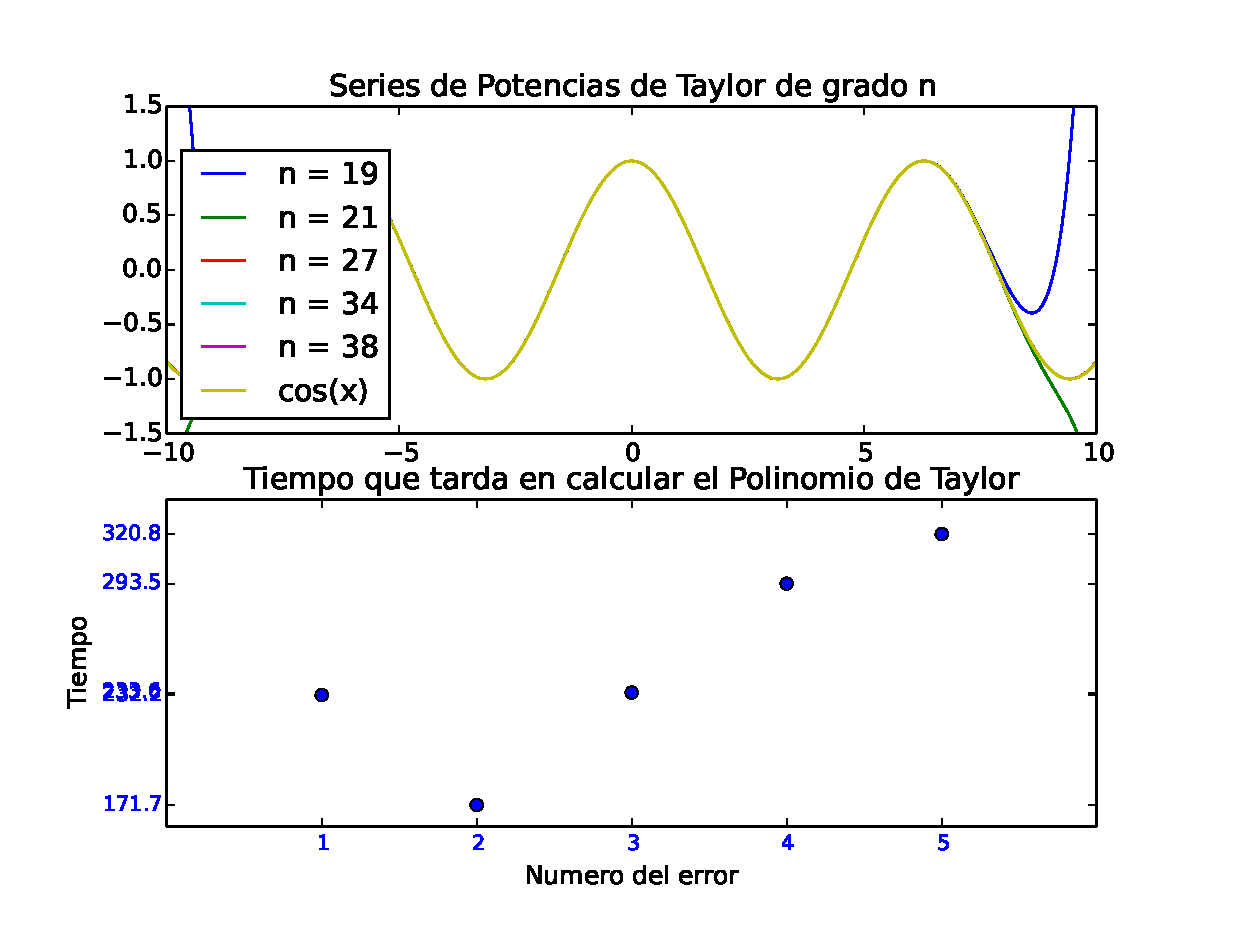
\includegraphics[height=5cm, width=6cm]{images/Graficas10.eps}
\caption{centro = 0; x = 10}
\label{cos}
\end{center}
\end{figure} 

\end{frame}  


%++++++++++++++++++++++++++++++++++++++++++++++++++++++++++++++++++++++++++++++

%\section{Bibliografía}
%++++++++++++++++++++++++++++++++++++++++++++++++++++++++++++++++++++++++++++++
%\begin{frame}
 % \frametitle{Bibliografía}

  %\begin{thebibliography}{10}
   

    %\beamertemplatebookbibitems
    %\bibitem{latex}
    % Wikipedia {\small http://es.wikipedia.org/wiki/Número\_$\pi$ }

    %\beamertemplatebookbibitems
    %\bibitem[URL: internet]{latex}
    %Logica {\small http://www.juegosdelogica.com/numero\_pi.htm}

  %\end{thebibliography}
%\end{frame}

%++++++++++++++++++++++++++++++++++++++++++++++++++++++++++++++++++++++++++++++
\end{document}